  % Chapter 5

\chapter{Numerical Results} \label{chap:NumericalResults}

In this chapter, we will apply a few selected mixed finite element pairs to several canonical test problems in order to learn how they might perform on real problems of engineering interest. 

\section{The Sod Shock Tube}
The Sod shock tube problem \cite{Sod1978} is a good starting point to check the ability of high order finite element pairs to model shock problems. The Sod shock tube is especially practical because it is one-dimensional, contains both shock waves and expansion fans, and can be solved exactly by means of a Riemann solver \cite{Toro2006}. The problem definition is of two initially static fluids of disparate pressures and densities in a shock tube. The diaphragm is burst, and the higher pressure gas on the left is allowed to expand into the lower pressure gas on the right. This forms two shock waves: one at the interface and the other within the lower density fluid, and one expansion fan in the high density fluid. Solid walls exist at $x=0$ and $x=1$ and the upper and lower boundaries are symmetry plains. The problem is allowed to run until $t=0.6$. The initial problem setup is illustrated in \refFig{SodShockTube}.

\begin{figure}[h!]
 \centering
 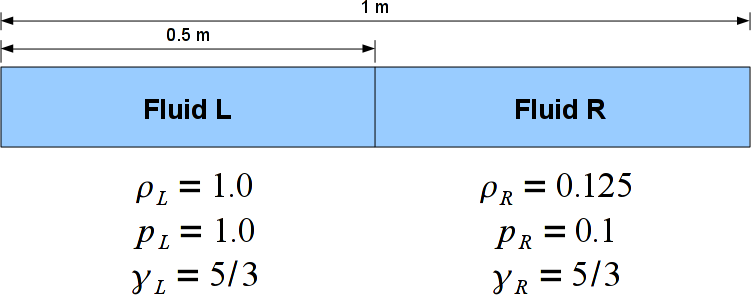
\includegraphics[width=5in,keepaspectratio=true]{./Figures/SodShockTube.png}
 % SodShockTube.png: 751x249 pixel, 107dpi, 17.82x5.91 cm, bb=0 0 505 167
 \caption{Problem setup for Sod shock tube problem}
 \label{fig:SodShockTube}
\end{figure}

For this one-dimensional problem, all higher order methods had nearly identical performance. Thus all of our comparisons will be between a single high-order method (\el{Q_2}{\hat Q_1}) and low order \el{Q_1}{Q_0} and assume that \el{Q_2}{\hat Q_2} would have performed similarly. Just to be absolutely clear, there a several little tweaks to \el{Q_1}{Q_0} that we could make to improve the solution, such as implementing a monotonic slope limiter \cite{BergerAftosmis05} or tuning of the \textsf{qquad} and \textsf{qlin} artificial viscosity coefficients. For our comparisons, we have put both elements on an equal footing by setting identical values of $\mathsf{qquad} = 1$ and $\mathsf{qlin}=1$. You will notice that both methods exactly capture the contact discontinuity. This is because the discontinuous nature of the thermodynamic basis functions makes multi-material physics natural and straightforward.

We can learn the most from a set of three plots. It is educational to consider \el{Q_1}{Q_0} on a refined mesh together with \el{Q_2}{\hat Q_1} on a course mesh. The higher-order \el{Q_2}{\hat Q_1} has twice as many DOFs in any direction as \el{Q_1}{Q_0}, so if we use 60 zones for \el{Q_2}{\hat Q_1} and 120 zones for \el{Q_1}{Q_0}, we will have the same total number of DOFs in the $x$-direction. Indeed, if we compare the blue and green lineouts in \refFig{SodCompare}, we see similar behavior despite the disparity in the mesh refinement. Thus we can understand that in general, for \el{Q_1}{Q_0} to achieve comparable accuracy to \el{Q_2}{\hat Q_1} we need twice as many zones in one dimension, four times as many in two dimensions, and eight times as many in three dimensions. This will be an important point when we consider the computational efficiency of each method. Furthermore, if we now consider \el{Q_2}{\hat Q_1} on the same refined mesh as \el{Q_1}{Q_0}, we see a significant improvement in accuracy. Please note the discontinuous behavior of the density plots. The $Q_0$ density climbs the shock in a series of flat steps while $\hat Q_1$ scales it with a smaller series of discontinuous line segments. 

These plots tell us some even more fundamental information about high order mixed finite elements than just accuracy. This first test problem demonstrates the practicality of using high order elements for shock problems. Our greatest fear was that Gibbs phenomenon \cite{Gibbs1898} would cause high frequency ringing around shock discontinuities for high order elements. We will see later that Gibbs phenomenon still occurs for high order elements, but this problem indicates that it may not be as significant an obstacle to overcome as we initially guessed.

\newpage
\begin{figure}[h!]
\begin{textblock*}{7.5in}(.5in,2in)
\centering
   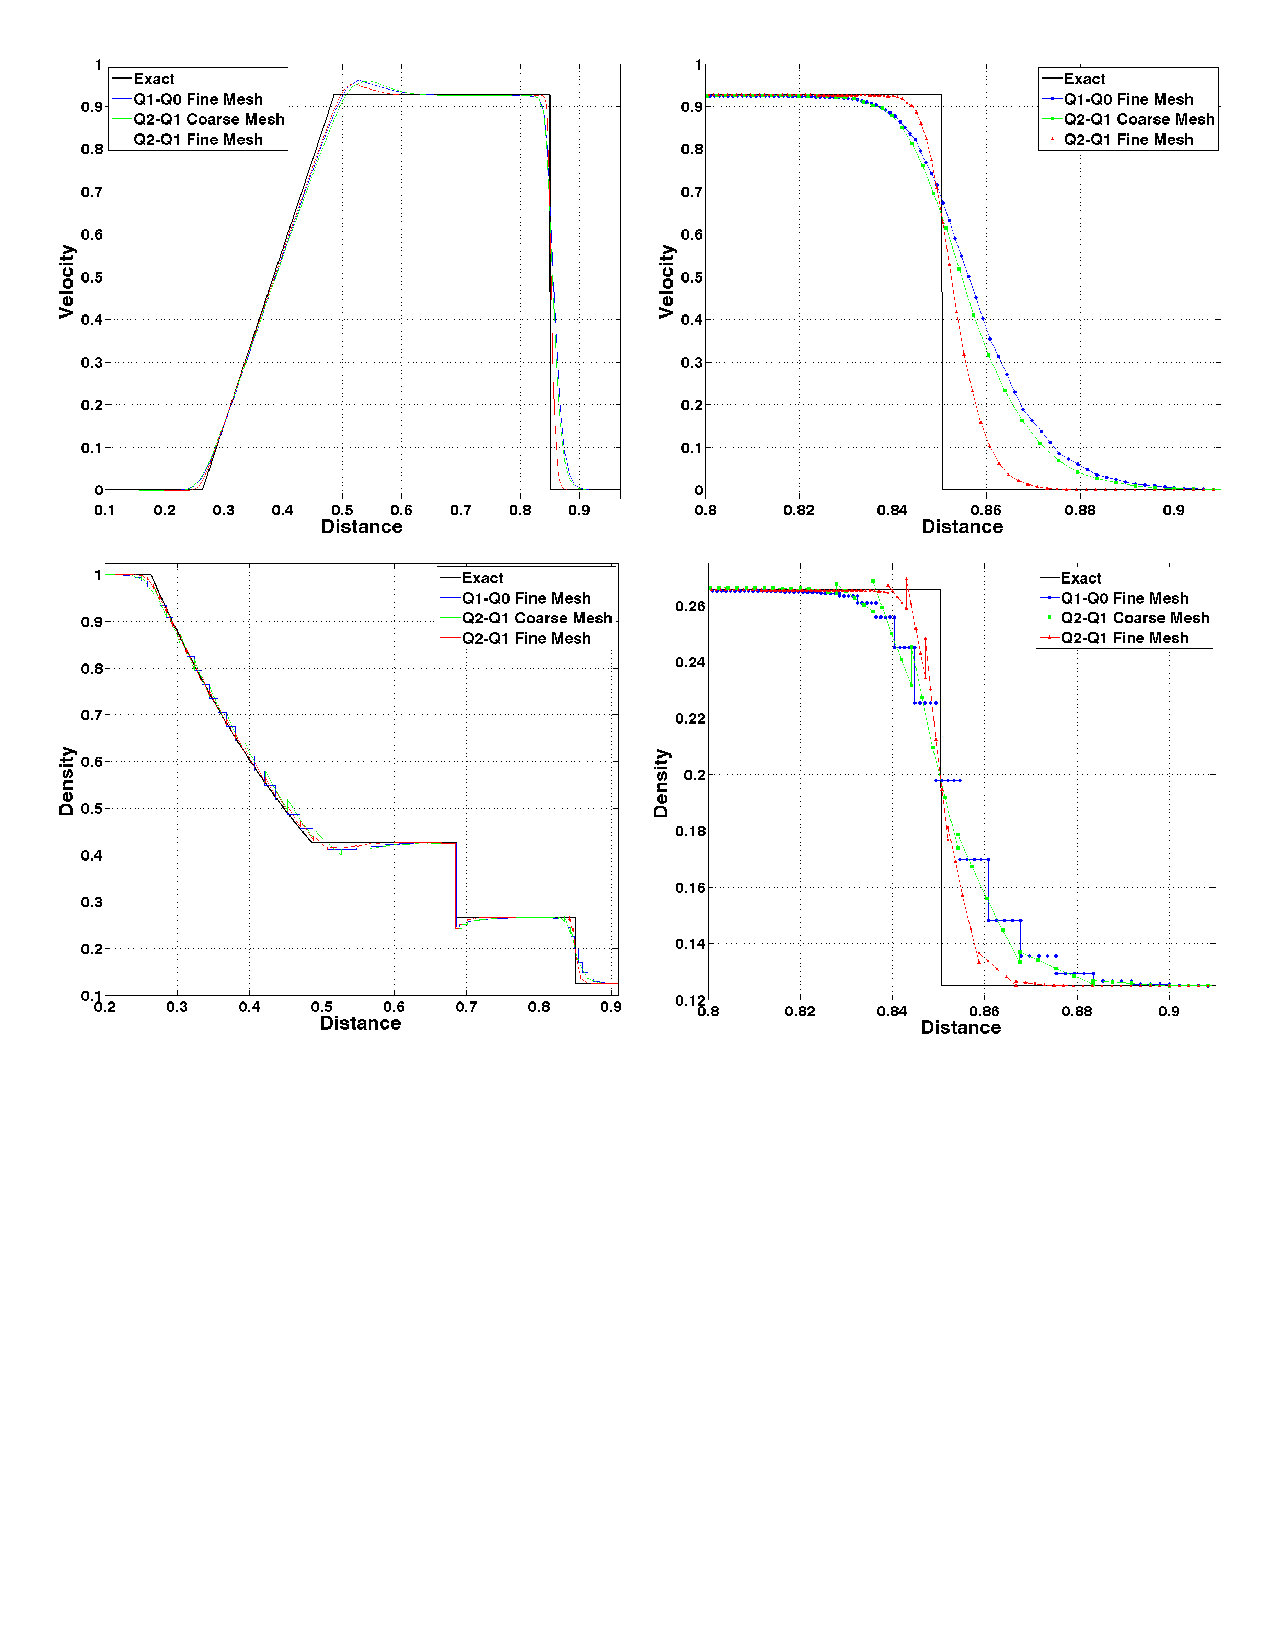
\includegraphics[trim = 0in 3.5in 0in 0in,clip,width=7.5in,keepaspectratio=true]{./Figures/SodCompare.pdf}
\end{textblock*}
\begin{textblock*}{5.5in}(1.5in,8.5in)
\caption{Comparison of \el{Q_1}{Q_0} and \el{Q_2}{\hat Q_1} elements on Sod shock tube and zoomed in on the shock (\textit{right}). Five plot points are considered per zone.}
 \label{fig:SodCompare}
\end{textblock*}
\end{figure}
\mbox{}\clearpage
\newpage

\section{The Noh Implosion}
The Noh implosion problem was first proposed by W. F. Noh \cite{Noh87}. This problem teaches us a lot about symmetry preservation of the method as well as accurate prediction of the shock speed and performance for a very strong shock (shock that decelerates gas to zero velocity). Historically, this problem has posed a significant challenge to bulk artificial viscosity formulations, as demonstrated by \refFig{Noh_MonoQ}, but we have built in the tensor artificial viscosity formulation of Campbell and Shashkov \cite{CampbellShashkov01} and formulated in a finite element sense by Kolev and Rieben \cite{KolevRieben09}. Thus, we should have little problem with symmetry breaking. Hourglass mode interference is minor or negligible for this problem, which allows us to experiment with a 2D shock problem without worrying too much about what effect the hourglass filter is having. In fact, we will be running all of the following cases without any hourglass filtering. Another useful characteristic of the Noh problem is that it has a simple analytical solution for all time, see below.

\begin{eqnarray*}
\vec V &=& \begin{cases}
\vec 0, &\text{for~}r\leq \frac{t}{3}\,, \\
-\hat r, &\text{for~}r > \frac{t}{3}\,.
\end{cases} \\
\rho &=& \begin{cases}
16, &\text{for~}r\leq \frac{t}{3}\,,\\
1 + \frac{t}{r}, &\text{for~}r > \frac{t}{3}\,.
\end{cases} \label{eq:NohAnalytical}\\
p &=& \begin{cases}
16/3, &\text{for~}r\leq \frac{t}{3}\,, \\
0, &\text{for~}r > \frac{t}{3}\,.
\end{cases} \\
\end{eqnarray*}


\begin{figure}[h!]
 \centering
 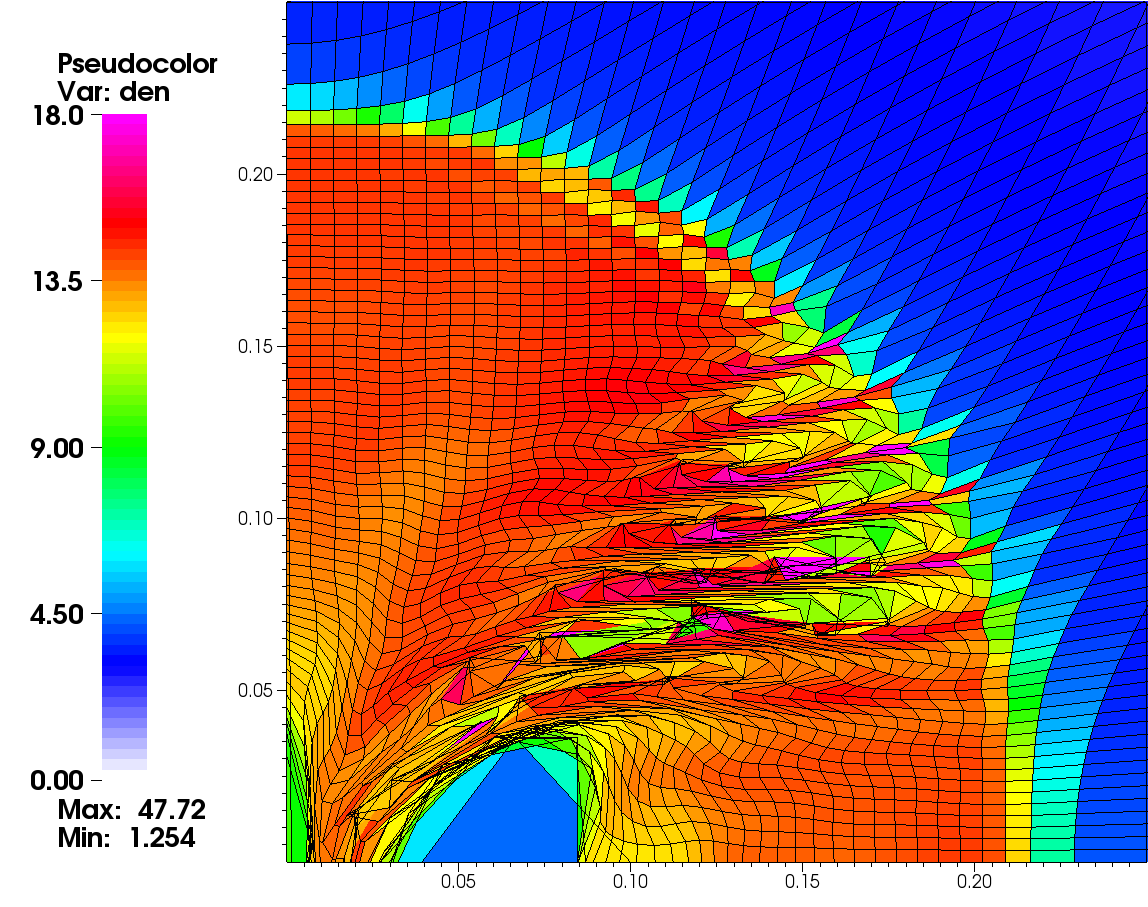
\includegraphics[width=5in,keepaspectratio=true]{./Figures/Noh2D_MonoQ.png}
 % SodShockTube.png: 751x249 pixel, 107dpi, 17.82x5.91 cm, bb=0 0 505 167
 \caption{Density pseudo-color at time t = 0.6 for the Noh problem on a 40 by 80 initial grid using the monotonic-scalar artificial viscosity.}
 \label{fig:Noh_MonoQ}
\end{figure}

The Noh problem is simple to set up. A uniform gas at zero pressure, with a density of 1.0 and $\gamma=5/3$ is initialized with a unit radially inward velocity at every point in the domain, as illustrated in \refFig{NohImplosion}. As the gas collides at the origin, the density builds up, and a shock wave expands radially outward at a speed of 1/3. There is one particular feature of this test problem that has plagued Lagrangian codes since its inception. ``Wall heating,'' which is caused by numerical shocks repeatedly reflecting through the zone at the origin causes that first cell to have a drastically lower density than it should \cite{Rider2000}. This is unavoidable for a simple research code such as \texttt{Fermium}, and is not a function of the finite element pair chosen, but purely of the framework (Eulerian or Lagrangian). We will just need to acknowledge its presence and then look past it.

It should be immediately obvious that we don't actually have to model this entire domain. One quadrant should be sufficient to obtain all the information we need. Therefore for this and the Sedov problem, we will only model the first quadrant and define the bottom and left boundaries to be symmetry plains. 

\begin{figure}[h!]
 \centering
 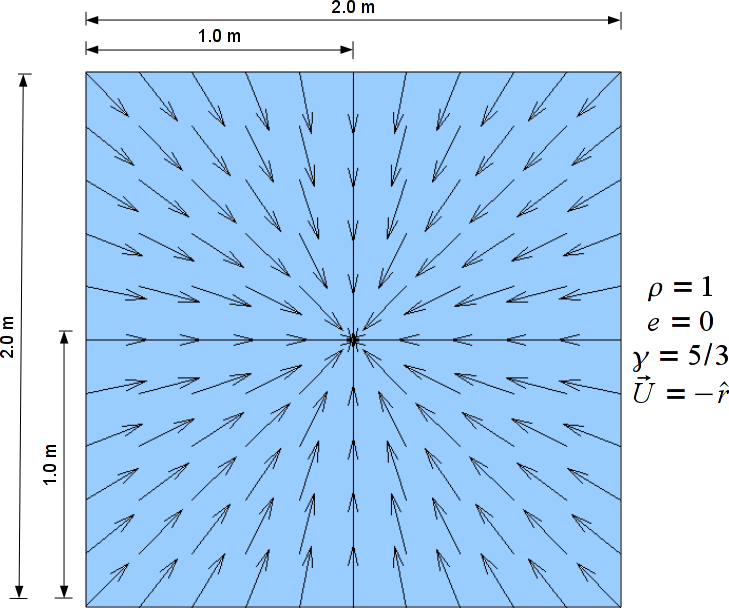
\includegraphics[width=3.5in,keepaspectratio=true]{./Figures/NohImplosion.png}
 % SodShockTube.png: 751x249 pixel, 107dpi, 17.82x5.91 cm, bb=0 0 505 167
 \caption{Problem setup for Noh implosion problem}
 \label{fig:NohImplosion}
\end{figure}

\subsection{Low Order \texorpdfstring{\el{Q_1}{Q_0}}{Q1-Q0}}
We require a huge number of low order elements to get anywhere close to the exact solution of the Noh problem. The original shock heating appears to irreparably damage the solution, dragging the predicted density way below the correct value and offsetting the shock past its correct position, see \refFig{Noh_Q1Q0_20x20_hgOFF}. The \el{Q_1}{Q_0} solution does have this going for it however, it does not undershoot or overshoot the solution at the shock front. This lends favorably to the stability of the method because we never see negative pressures or densities show up in the solution. We also consider a refined 40$\times$40 solution in \refFig{Noh_Q1Q0_40x40_hgOFF} in order to observe the convergence to the analytical solution.

\NohPlot{Q1Q0}{20}{OFF}{\el{Q_1}{Q_0}}{without}
\NohPlot{Q1Q0}{40}{OFF}{\el{Q_1}{Q_0}}{without}

\subsection{Low Order \texorpdfstring{\el{Q_1}{\hat Q_1}}{Q1-Q1}}
Now turning to the \el{Q_1}{\hat Q_1} element, we can see some promising results from the Noh problem, as illustrated by \refFig{Noh_Q1Q1_20x20_hgOFF}. We still don't achieve the desired post-shock density, but the solution looks very reasonable and stable overall. The post-shock density field looks especially uniform compared to \el{Q_2}{\hat Q_1} and \el{Q_2}{\hat Q_2}. Even with the refined 40$\times$40 mesh, the density doesn't quite reach the correct value, but the field is pretty good overall. Sharing the same kinematic basis functions, the velocity field is very similar to \el{Q_1}{Q_0}.

\NohPlot{Q1Q1}{20}{OFF}{\el{Q_1}{\hat Q_1}}{without}
\NohPlot{Q1Q1}{40}{OFF}{\el{Q_1}{\hat Q_1}}{without}

\subsection{High Order \texorpdfstring{\el{Q_2}{\hat Q_1}}{Q2-Q1}}
We see a marked improvement when we switch to higher order, as illustrated by \refFig{Noh_Q2Q1_20x20_hgOFF}. Both the velocity and density plots get a lot closer to the exact solution, but we also start to see some troubling features. The density scatter plot shows some huge overshoots and undershoots oscillating around the shock front, we also get some small overshoots in the velocity plot. This is slightly troubling because we actually see density dip below the x-axis to some negative values. The average density in each cell would still be positive, but even a negative interpolation is cause for concern. Indeed, it is very important that we address this if we ever wish to implement a high-order Lagrangian hydro code. We have observed that this oscillation can be controlled through adjustment of the artificial viscosity coefficients, but this also significantly smears out the shock. The concept of hyperviscosity, as postulated by Cook and Cabot \cite{CookCabot2004,CookCabot2005} shows particular promise at eliminating shock oscillations for higher order methods. This method uses multiplications of the stiffness matrix to filter out non-physical oscillatory behavior with a minimal number of problem dependent constants. Please note the significant improvement in the matching capability of the density plot. While a 40$\times$ by \el{Q_1}{Q_0} mesh fails to accurately predict the post-shock density, a mere 20$\times$20 \el{Q_2}{\hat Q_1} hits it right on the head. Although the oscillations get worse under refinement, the overall solution gets much closer to the analytic prediction under refinement as we can see in \refFig{Noh_Q2Q1_40x40_hgOFF}. The velocity matching is the closest of anything that we have seen so far. 

\NohPlot{Q2Q1}{20}{OFF}{\el{Q_2}{\hat Q_1}}{without}
\NohPlot{Q2Q1}{40}{OFF}{\el{Q_2}{\hat Q_1}}{without}

\subsection{High Order \texorpdfstring{\el{Q_2}{\hat Q_2}}{Q2-Q2}}\label{sec:nohQ2Q2}
The benefit of this element chiefly lies in its ability to avoid density undershoots at the shock front. The bi-quadratic density and pressure fields must give a single element the flexibility to jump from a low to a high density  without overshooting both directions while still maintaining the correct mass within that zone. The density overshoots on the other hand, are more more severe than the \el{Q_2}{\hat Q_1} element. The velocity field is much the same as its \el{Q_2}{\hat Q_1} cousin.

\NohPlot{Q2Q2}{20}{OFF}{\el{Q_2}{\hat Q_2}}{without}
\NohPlot{Q2Q2}{40}{OFF}{\el{Q_2}{\hat Q_2}}{without}

\section{The Saltzman Piston}
The Saltzman piston problem \cite{Saltzman1985,Gryra1992} is commonly used to test the effectiveness of new artificial viscosity schemes. In this problem a one-dimensional piston driven shock propagates through a two-dimensional mesh that has been perturbed according to \refEq{SaltzmanPert}. We applied this transformation to a 50$\times$10 mesh with original width and height of 1.0 and 0.1, as shown in \refFig{SaltzmanMesh}. This tests the ability of a method to model shock waves that are not aligned with the mesh. The tensor artificial viscosity formulation has already been tested on the Saltzman piston by  \cite{CampbellShashkov01},  \cite{KolevRieben09}, and  \cite{Lipnikov2010}, but we aim to demonstrate the effectiveness of high order elements on this problem.

\newEq{SaltzmanPert}{
x(i,j)=(i-1)\frac{x_{max}-x_{min}}{NZ_x}+(NZ_y+1-j)\sin\left(\frac{\pi(i-1)}{NZ_x}\right)\frac{y_{max}-y_{min}}{NZ_y}}

\begin{figure}[h!]
 \centering
 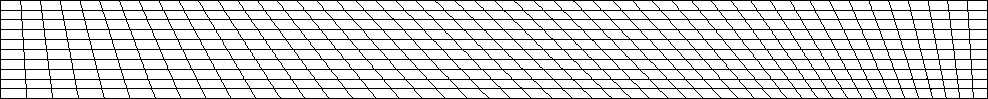
\includegraphics[width=6in,keepaspectratio=true]{./Figures/SaltzmanMesh2.png}
 % SodShockTube.png: 751x249 pixel, 107dpi, 17.82x5.91 cm, bb=0 0 505 167
 \caption{Initial perturbed Saltzman piston mesh}
 \label{fig:SaltzmanMesh}
\end{figure}

The domain is initially filled with an ideal gas ($\gamma=5/3$) of density 1 and zero pressure. A piston enters from the left side at a constant speed of 1.0 which generates a shock that reaches the right wall at $t=0.8$ and reflects off the left wall again at $t=0.9$. We run the simulation to a time of 0.925 which stops the simulation shortly before the shock reaches the right wall a second time. The analytical pre- and post-shock densities are 10 and 20, respectively. Similar to Noh, this problem also suffers from ``wall heating'' and the low right and left densities should be overlooked. 

\subsection{Low Order \texorpdfstring{\el{Q_1}{Q_0}}{Q1-Q0}}
The tensor artificial viscosity allows this solution to progress smoothly without the mesh tangling that we see with bulk artificial viscosity formulations \cite{Barlow07}. The shock front is a little jagged because the shock must tackle a whole piece-wise constant density cell at a time rather than smoothly traversing it with a bi-linear or bi-quadratic thermodynamic interpolation. Thus the shock gets ahead of itself at points and behind in others. When we look at the hourglass filtered solution, we see our first evidence that hourglass filters should not be arbitrarily applied with equal magnitude to every problem. They must be tuned for each simulation, and herein lies their Achilles heel. The simulationist must invest a significant amount of time running and rerunning any new problem to determine the optimal hourglass filter setting. We seek either a filter that does not require tuning or preferably an element pair that will be naturally hourglass free. We have not yet arrived at a suitable solution. \refFig{Saltzman_Q1Q0_50x10_hgON} demonstrates that an hourglass filter can do more to harm a solution than to fix it. Even without an hourglass filter, we see some post-shock waves in the mesh where we should see horizontal lines.

\SaltzmanPlot{Q1Q0}{}{OFF}{\el{Q_1}{Q_0}}{without}
\SaltzmanPlot{Q1Q0}{}{ON}{\el{Q_1}{Q_0}}{with}

\subsection{Low Order \texorpdfstring{\el{Q_1}{\hat Q_1}}{Q1-Q1}}
We get some very positive results when we update to a bi-linear thermodynamic space. The additional pressure and density information allows the shock to move through the domain with less interference to the mesh. In \refFig{SaltzmanD_Q1Q1_50x10_hgOFF} we can see certain zones partly shocked while one corner remains in its pre-shock condition. Similar to \el{Q_1}{Q_0}, we also see some incorrect post-shock waves in the mesh. Overall, however, this is a very solid solution.

\SaltzmanPlot{Q1Q1}{}{OFF}{\el{Q_1}{\hat Q_1}}{without}
% \SaltzmanPlot{Q1Q1}{}{ON}{\el{Q_1}{\hat Q_1}}{with}

\subsection{High Order \texorpdfstring{\el{Q_2}{\hat Q_1}}{Q2-Q1}}
Looking primarily at the mesh, \el{Q_2}{\hat Q_1} produces the best solution so far. The horizontal mesh lines are straighter than and the shock more uniform than any of the lower order results. The shock has a lot more flexibility to travel unimpeded across each cell layer because of high order information within each zone. The shock itself is very sharp with some velocity overshoots and significant density overshoots. The chief failing of this method is in the manifestation of the hourglass modes. Indeed, this simulation will not run to completion without an hourglass filter. We see the opposite scenario with the Sedov problem - \el{Q_1}{Q_0} will not run without and hourglass filter, but \el{Q_2}{\hat Q_1} will. This further illustrates the unpredictable nature of hourglass modes. It is very hard to tell if and when they will throw a wrench in a simulation. 

\SaltzmanPlot{Q2Q1}{}{ON}{\el{Q_2}{\hat Q_1}}{with}

\subsection{High Order \texorpdfstring{\el{Q_2}{\hat Q_2}}{Q2-Q2}}
A higher order thermodynamic field allows us to run the simulation to completion without an hourglass mode, but we still see evidence of near failure at the shock front near the top surface. A near mesh-collapse has produced a ``hot spot'' of very high density and pressure. Aside from this, the mesh looks very good with relatively straight horizontal mesh lines. We get a more stable solution with an hourglass filter except for an anomalous ``cold spot'' in the center of the post-shock velocity field. With an hourglass filter, the overall solution appears to be superior to the low order methods but inferior to the \el{Q_2}{\hat Q_1} results with an hourglass filter. 

\SaltzmanPlot{Q2Q2}{}{OFF}{\el{Q_2}{\hat Q_2}}{without}
\SaltzmanPlot{Q2Q2}{}{ON}{\el{Q_2}{\hat Q_2}}{with}

\section{The Sedov Blast Wave}
The previous problems were informative, but they did not allow us to demonstrate the true power of high order elements - curvilinear zones. The Sedov explosion problem \cite{Sedov59} brings these curvilinear capabilities to the forefront. In two dimensions, the Sedov problem is a point-blast wave in an initially static ideal gas medium of constant density, zero pressure, with a delta function initial source of energy at the origin, as illustrated in \refFig{SedovExplosion}. In plain terms, this a simplification of an explosion: a lot of energy is released in a small area and then it expands into the surrounding domain. The problem runs to $t$=1.0 which allows the shock wave to expand to a radius of 1.0.

\begin{figure}[h!]
 \centering
 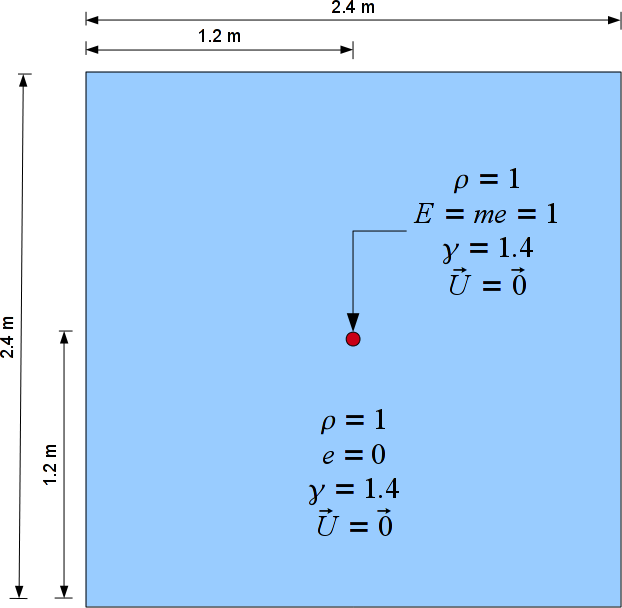
\includegraphics[width=3in,keepaspectratio=true]{./Figures/SedovExplosion.png}
 % SodShockTube.png: 751x249 pixel, 107dpi, 17.82x5.91 cm, bb=0 0 505 167
 \caption{Problem setup for Sedov blast wave problem}
 \label{fig:SedovExplosion}
\end{figure}

We mentioned previously that the Sedov blast wave presents one of the most compelling arguments for using curvilinear elements. By its very nature, this problem seeks to curve geometries that may have been initially Cartesian. Indeed, when we apply the exact solution of this problem to an initially Cartesian grid, as we do in \refFig{CartSedov}, it becomes obvious that anything other than curvilinear elements would introduce undesirable inaccuracies into the mesh geometry, even under refinement.

\begin{figure}[h!]
 \centering
 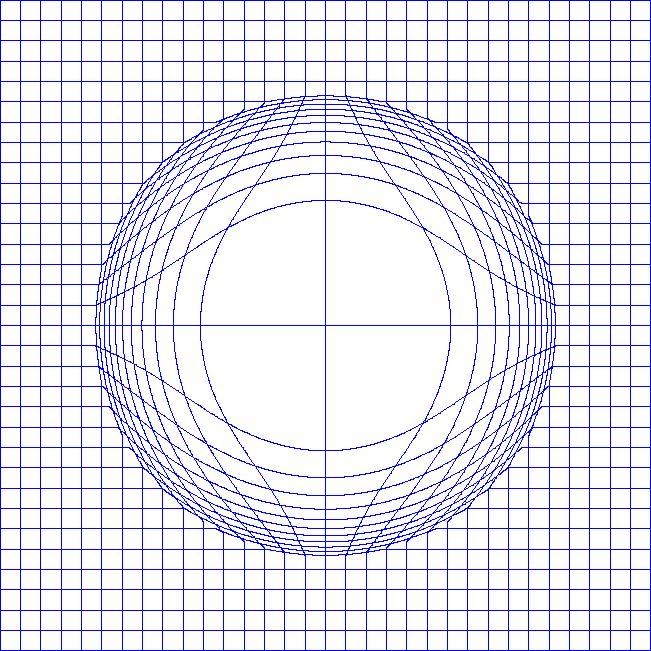
\includegraphics[width=5in,keepaspectratio=true]{./Figures/sedovCart.png}
 % SodShockTube.png: 751x249 pixel, 107dpi, 17.82x5.91 cm, bb=0 0 505 167
 \caption{Exact solution to the Sedov problem applied to an initially Cartesian grid}
 \label{fig:CartSedov}
\end{figure}

\subsection{Low Order \texorpdfstring{\el{Q_1}{Q_0}}{Q1-Q0}}
Historically, this problem has presented significant challenges to \el{Q_1}{Q_0} because hourglass mode instabilities cause the solution to crash if they are not filtered out. We would like to compare each of our methods with and without an hourglass filter, but it is simply impossible to obtain an hourglass filter-less solution with \el{Q_1}{Q_0}. If we do apply an hourglass filter we are able to get a stable solution, as seen in\refFig{Sedov_Q1Q0_10x10_hgON} with a very coarse 10$\times$10 mesh.

The Sedov problem is inherently circular. A point source of energy should produce a circular blast wave expanding out from the origin. Therein we see a significant limitation of low order methods. We are only able to produce straight-edged elements with \el{Q_1}{Q_0} which interfere with the curved nature of the problem. With this coarse mesh we can see how the zone at the origin (which doesn't have enough DOFs to represent a curved edge) induces an kinked shock wave where we should see a nice smooth radius. This problem can be mitigated by adding more elements, but it still exists as a significant source of error when modeling fundamentally curved phenomena.

You will also notice that the shock has been smeared considerably. This is primarily the fault of the piece-wise constant representation for density and pressure. We can thank artificial viscosity for smoothing the shock discontinuity out enough to allow a numerical solution, but we still expect to see sharp gradients of density, pressure, and velocity. The low order method can only take one step in density or pressure per zone, thus we see the shock being spread over several zones to smooth out the sharp change in value. We can alleviate this shock smoothing by tweaking the artificial viscosity coefficients, but the fact remains that low order methods are fundamentally limited in their ability to capture sharp gradients.

This low order representation of density and pressure also limits our ability to accurately predict the maximum density and pressure in the shock wave. The constant density interpolation is only able to represent averages over a zone without any additional fluctuations within that zone. Thus, for rapidly changing phenomena like a blast wave, we are very limited in what we can learn without extensive mesh refinement.

We are able to see nominal improvement if we double the resolution in both the $x$- and $y$- directions, as seen in \refFig{Sedov_Q1Q0_20x20_hgON}. While higher resolution attains closer correspondence to the exact solution, the density spike is still grossly under-predicted, and the zone at the origin is still fails to resemble the exact solution in \refFig{CartSedov}.

\SedovPlot{Q1Q0}{10}{ON}{\el{Q_1}{Q_0}}{with}
\SedovPlot{Q1Q0}{20}{ON}{\el{Q_1}{Q_0}}{with}

\subsection{Low Order \texorpdfstring{\el{Q_1}{\hat Q_1}}{Q1-Q1}}
As discussed previously, the main benefit of the \el{Q_1}{\hat Q_1} element is that it appears to squelch hourglass modes in certain situations. We saw in \refSec{Q1Q1spuriousmodes} that this element introduces new spurious modes, but in the Sedov problem, at least, these modes appear to be negligible. The immediate improvement we see when we compare the 10$\times$10 results to \el{Q_1}{Q_0} is that the higher order density field allows the shock to better maintain a circular shape. This results in a more tightly grouped, and hence more accurate, velocity scatter plot. The density results also adhere more closely to the exact solution, approaching closer to the peak value. Despite the straight-edged zones, this is a very good solution overall, and it only gets better with more elements. The shock is still more blurred than higher order methods can give us and the density still does not quite reach the accurate peak value.

\SedovPlot{Q1Q1}{10}{OFF}{\el{Q_1}{\hat Q_1}}{without}
\SedovPlot{Q1Q1}{20}{OFF}{\el{Q_1}{\hat Q_1}}{without}

\subsection{High Order \texorpdfstring{\el{Q_2}{\hat Q_1}}{Q2-Q1}}
The most prominent feature of the \el{Q_2}{\hat Q_1} solution is the curved original zone. Without an hourglass filter it looks almost as if it were bowing out from the force of the explosion. This bowing is actually non-physical, but the overall curvature of the element lends very favorably to the accuracy of the scheme. We also see post-shock oscillations in the velocity field. Despite these hourglass-based penalties, the shock capturing is much sharper. At many points we can see the entire shock captured within one zone. 

If we apply a simple hourglass filter by leaving 25\% of linear artificial viscosity term on in expansion, the results look very fine indeed. The curved zones are reminiscent of the exact solution of the mesh geometry in \refFig{CartSedov}. This also eliminates the oscillations and gives us a solution very close the exact. The results only get better under refinement. At 20$\times$20 mesh refinement, we see very little variation from the exact answer.

In order to completely level the playing field concerning the limitations of \el{Q_1}{Q_0} for curved geometries, we should consider the same problem using the same number of DOFs with curvilinear elements. One of the most significant limitations of low order elements on the Sedov problem was that for a coarse enough grid (10$\times$10), the zone at the origin induced a kinked shape on the shock wave downstream. If we wish to compare this result with curvilinear elements with the same number of DOFs, we would need to use the almost absurd mesh resolution of 5$\times$5. We can see in \refFig{Sedov_Q2Q1_5x5_hgON} that this coarse \el{Q_2}{\hat Q_2} solution avoids the angular mesh problem and produces a surprisingly symmetric and reasonable result.

\SedovPlot{Q2Q1}{10}{OFF}{\el{Q_2}{\hat Q_1}}{without}
\SedovPlot{Q2Q1}{10}{ON}{\el{Q_2}{\hat Q_1}}{with}
\SedovPlot{Q2Q1}{20}{ON}{\el{Q_2}{\hat Q_1}}{with}

\SedovPlot{Q2Q1}{5}{ON}{\el{Q_2}{\hat Q_1}}{with}

We gain some further insight when we run this simulation on a full mesh, and instead of splitting up the energy source into four cells, we energize a single cell which encompasses the origin. We can see the results of two 21$\times$21 runs in \refFig{SedovFullMeshCompare}. The \el{Q_1}{Q_0} elements lack the flexibility to expand naturally from the force of the explosion, hence the original zone is forced to retain its square shape as it expands. This imposes a square shock front and causes the corner elements to bend unnaturally until one of the corners exceeds a 180 degrees at $t$=0.868. This causes the Jacobian to go negative and the solution to go unstable and the simulation to stop. The bi-quadratic method, on the other hand, possesses the required flexibility to expand naturally with the force of the explosion, and the simulation progresses smoothly to the end at $t$=1.0. This is a rather extreme test, but curvilinear elements displays a distinct advantage of straight-edged methods. 

\begin{figure}[h!]
 \centering
 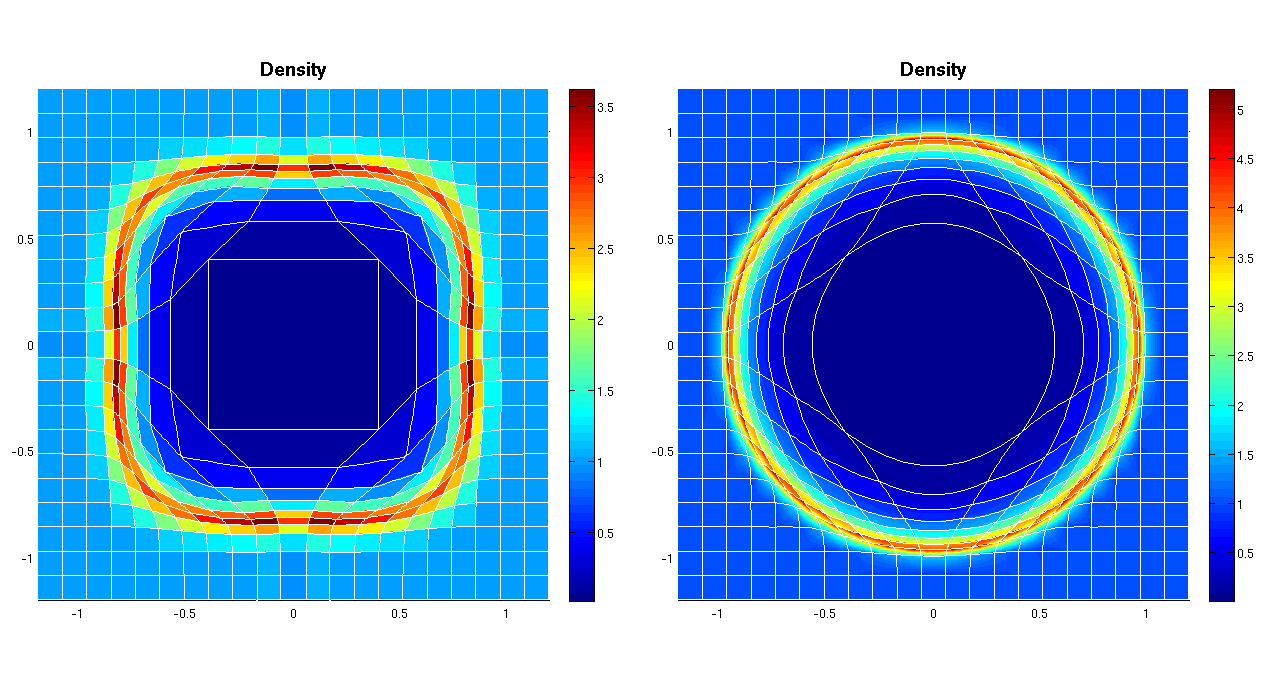
\includegraphics[width=6in,keepaspectratio=true]{./Figures/SedovFullMeshCompare.png}
 % SodShockTube.png: 751x249 pixel, 107dpi, 17.82x5.91 cm, bb=0 0 505 167
 \caption{Comparison of \el{Q_1}{Q_0} (\textit{left}) and \el{Q_2}{\hat Q_1} (\textit{right}) on a full 21$\times$21 mesh.}
 \label{fig:SedovFullMeshCompare}
\end{figure}

% \clearpage
% \newpage
% \begin{figure}[ht]
% \begin{textblock*}{7in}(.75in,1in)
% \centering
% \subfigure[Velocity magnitude pseudocolor plot (\textit{left}). Velocity magnitude scatter plot compared to exact solution (\textit{right}).]{
% 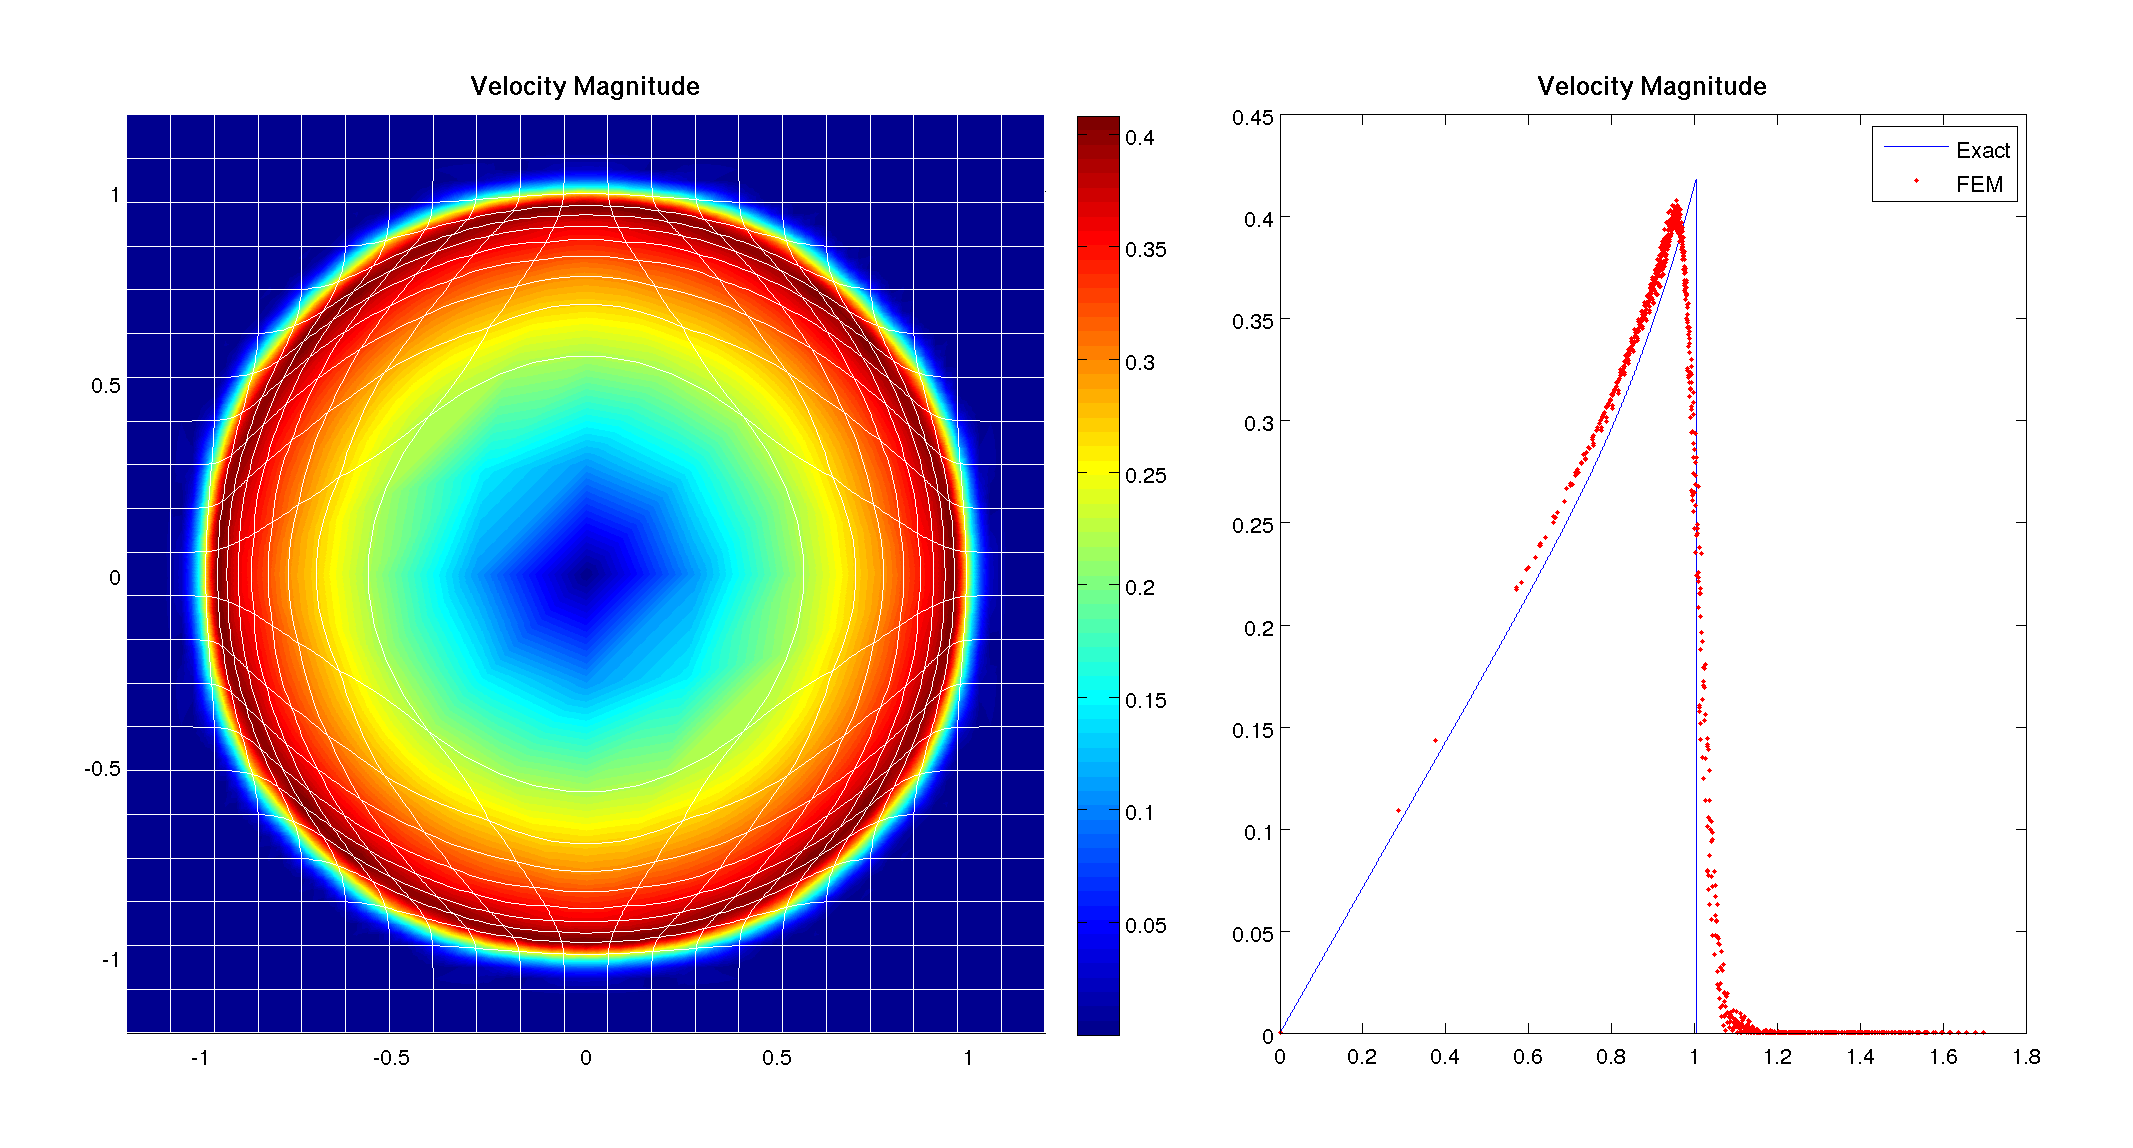
\includegraphics[width=7in,keepaspectratio=true]{./Figures/FullMesh/SedovV_Q2Q1_21x21_hgON}
% \label{fig:SedovV_#1_#2x#2_hg#3}
% }
% \subfigure[Density pseudocolor plot (\textit{left}). Density scatter plot compared to exact solution (\textit{right}).]{
% 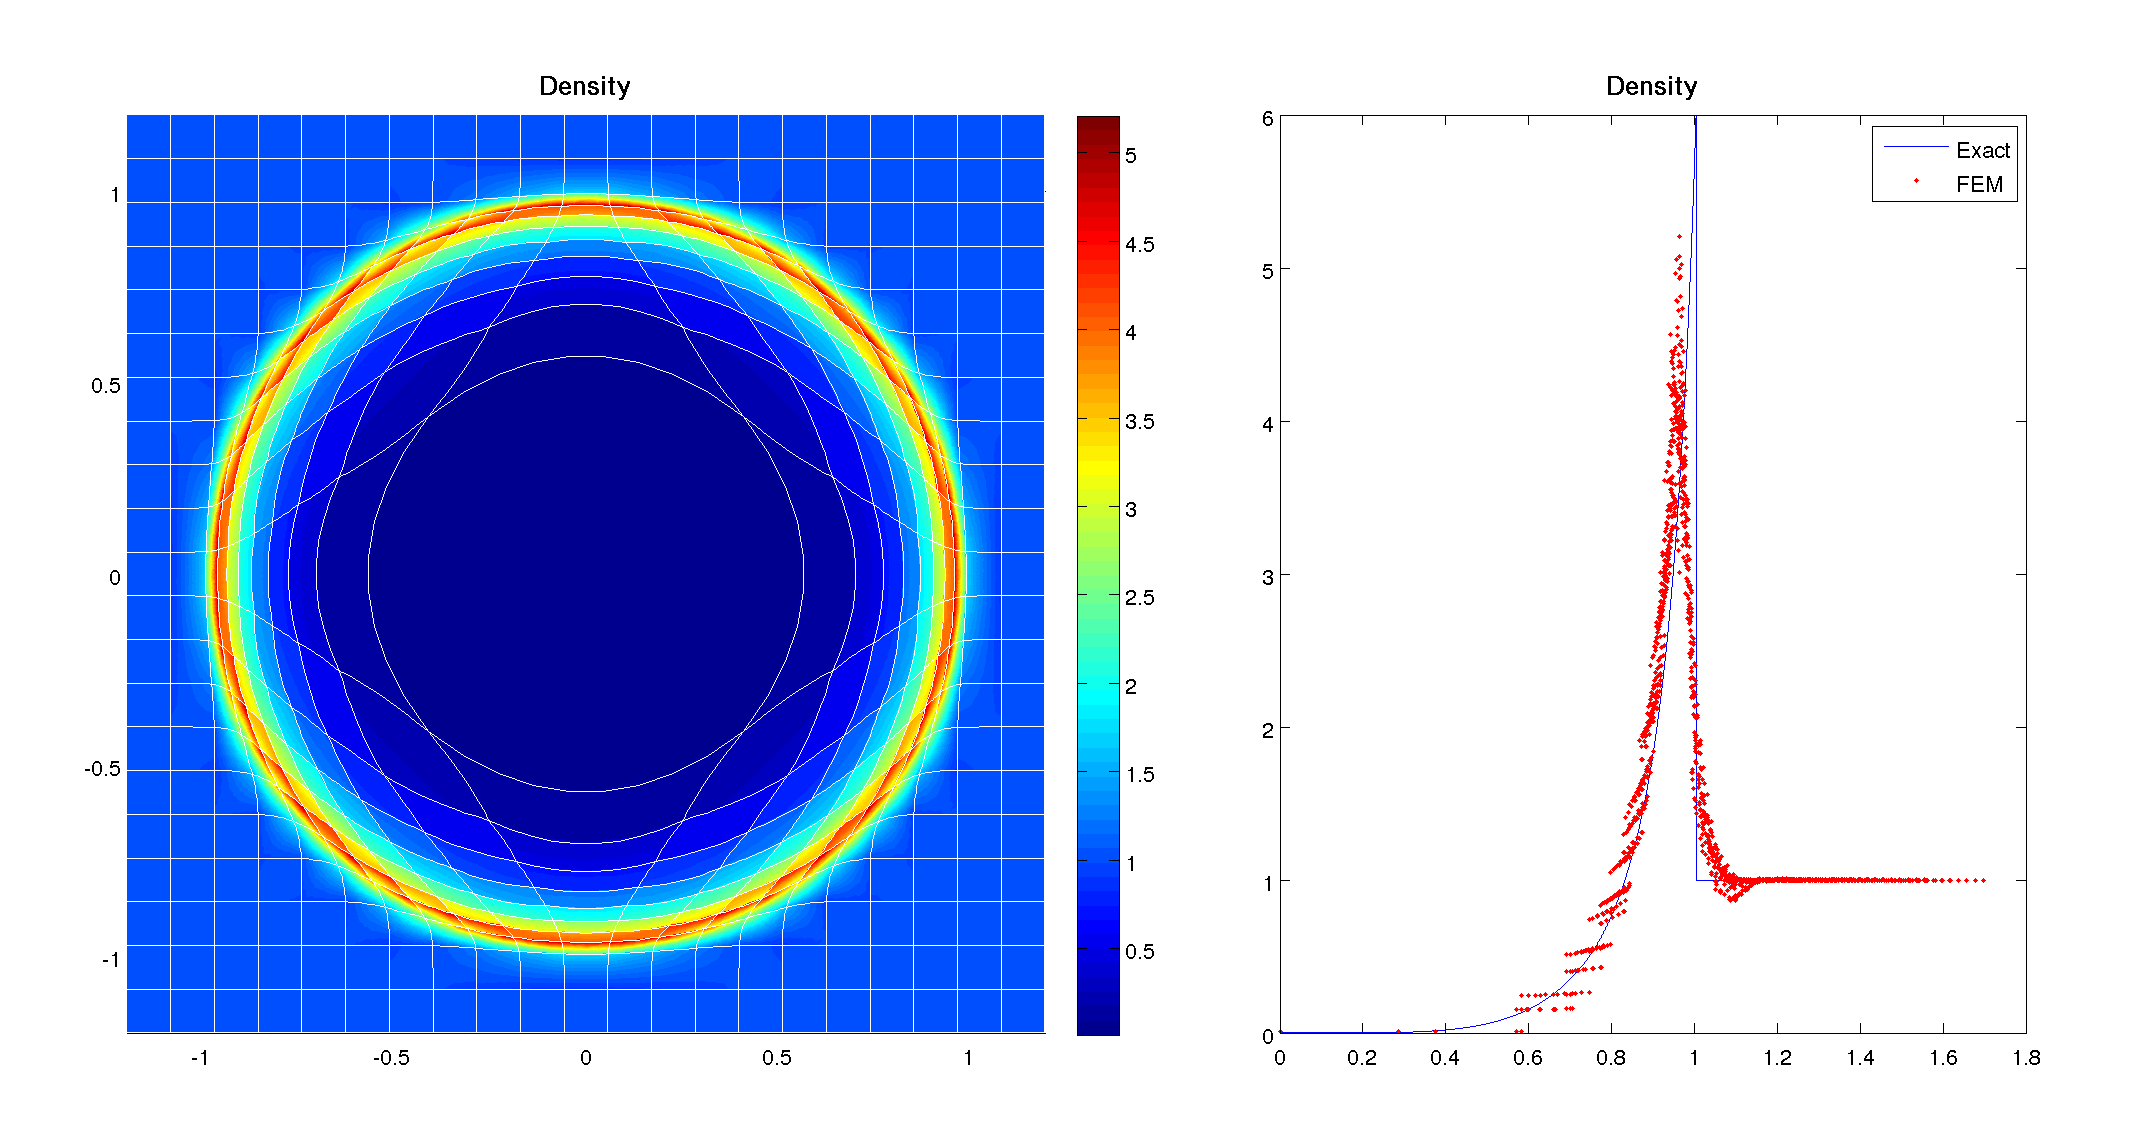
\includegraphics[width=7in,keepaspectratio=true]{./Figures/FullMesh/SedovD_Q2Q1_21x21_hgON}
% \label{fig:SedovD_#1_#2x#2_hg#3}
% }
% \caption{Sedov explosion problem on 21$\times$21 full mesh using \el{Q_2}{\hat Q_1} elements with hourglass filtering}
% \label{fig:Sedov_#1_#2x#2_hg#3}
% \end{textblock*}
% \end{figure}
% \clearpage
% \newpage

\subsection{High Order \texorpdfstring{\el{Q_2}{\hat Q_2}}{Q2-Q2}}
\el{Q_2}{\hat Q_2} does not perform quite as admirably for this problem. Without an hourglass filter we get some velocity ``hot spots'' at the symmetry boundaries and despite its higher order potential, the original zone is not nearly curved enough. It almost looks like one of the lower order solutions. The situation actually gets worse under refinement. The original cell and many layers beyond actually bow inward, a phenomenon that is completely non-physical. We also start to see some very bad noise in the velocity plot. This just goes to show the unpredictable nature of the \el{Q_2}{\hat Q_2} element. In some cases it appears to squelch hourglass modes, but in others spurious modes run rampant. The solution improves dramatically with an hourglass filter.

\SedovPlot{Q2Q2}{10}{OFF}{\el{Q_2}{\hat Q_2}}{without}
% \SedovPlot{Q2Q2}{10}{ON}{\el{Q_2}{\hat Q_2}}{with}
\SedovPlot{Q2Q2}{20}{OFF}{\el{Q_2}{\hat Q_2}}{without}
\SedovPlot{Q2Q2}{20}{ON}{\el{Q_2}{\hat Q_2}}{with}


\section{Computational Efficiency}
The fairest comparison of computational efficiency is to compare the runtimes of several solutions using the same number of kinematic degrees of freedom. Thus a 5$\times$5 \el{Q_2}{\hat Q_1} mesh would have the same number of kinematic degrees of freedom as a 10$\times$10 \el{Q_1}{Q_0} mesh. By the related nature of these two elements, the number of thermodynamic DOFs is also the same between these two meshes. High order methods become computationally attractive when we take this viewpoint. Most of the steps in the solution process proceed one-by-one through each element. If we can limit the number of zones that we loop through and distribute more work to each element, we can drastically improve the performance of the code. We ran the Sedov and Noh problems at a variety of mesh resolutions for all four methods that we have been considering and compiled the results in \refTab{SedovRunTime} and \refTab{NohRunTime}. It appears that higher order \el{Q_2}{\hat Q_1} levels off at approximately twice as fast per degree of freedom as \el{Q_1}{\hat Q_0}.

\begin{table}[!ht]
\caption{Sedov run times compared across the number of kinematic degrees of freedom. Time in seconds. \newline}\label{tab:SedovRunTime}
\begin{tabular}[c]{|c|cc|cc|cc|}
\hline
Method & \multicolumn{2}{|c|}{36 Degrees of Freedom} & \multicolumn{2}{|c|}{121 Degrees of Freedom} & \multicolumn{2}{|c|}{441 Degrees of Freedom}\\
\hline
 & Run Time & Speedup & Run Time & Speedup & Run Time & Speedup\\
\el{Q_1}{Q_0} & 28.154 & 1.0 & 156.021 & 1.0 & 1265.232 & 1.0 \\
\el{Q_1}{\hat Q_1} & 29.565 & 0.95 & 165.185 & 0.94 & 1291.628 & 0.98 \\
\el{Q_2}{\hat Q_1} & 16.328 & 1.72 & 73.375  & 2.13 & 623.658 & 2.03 \\
\el{Q_2}{\hat Q_2} & 17.017 & 1.65 & 77.632  & 2.01 & 663.122 & 1.91 \\
\hline
\end{tabular}
\end{table}

\begin{table}[!ht]
\caption{Noh run times compared across the number of kinematic degrees of freedom. Time in seconds. \newline}\label{tab:NohRunTime}
\begin{tabular}[c]{|c|cc|cc|cc|}
\hline
Method & \multicolumn{2}{|c|}{36 Degrees of Freedom} & \multicolumn{2}{|c|}{121 Degrees of Freedom} & \multicolumn{2}{|c|}{441 Degrees of Freedom}\\
\hline
 & Run Time & Speedup & Run Time & Speedup & Run Time & Speedup\\
\el{Q_1}{Q_0}      & 101.192 & 1.0 & 383.356 & 1.0 & 1543.319 & 1.0 \\
\el{Q_1}{\hat Q_1} & 103.048 & 0.98 & 396.967 & 0.97 & 1590.766 & 0.97 \\
\el{Q_2}{\hat Q_1} & 53.042 & 1.91 & 191.063  & 2.01 & 775.230 & 1.99 \\
\el{Q_2}{\hat Q_2} & 53.605 & 1.89 & 194.381  & 1.97 & 792.363 & 1.95 \\
\hline
\end{tabular}
\end{table}

When we run a profile of our code, it appears that the largest chunk of computer time is spent on the high order Jacobian calculation. This makes sense because this function is evaluated once per quadrature point per zone per time step, and this is a somewhat complicated matrix to calculate. But from our results above, it appears that even a full bi-quadratic Jacobian matrix is not enough to slow this method down appreciably.

When we couple the faster run times with the fact that higher order methods converge to lower errors with fewer elements, high order methods become very computationally attractive. 